\section{Results and Analysis}
\label{sec:results}

The descriptive comparison (Table~\ref{tab:main-results}) reports completed extraction systems, with strict scores kept separate from a detection diagnostic. Full breakdowns and paired intervals appear in \S\ref{app:result-layout}. Figure~\ref{fig:context-contrasts} visualizes the ten completed within-model comparisons.

\begin{table}[t]
\caption{Completed-run scores (0--100). Strict is end-to-end exact F1; D is the post-hoc detection proxy with invalid-item penalties. F/L: full/local. Baselines occupy Strict-F as document-level references, not a context pair. --: no completed condition or not applicable. $\dagger$: 1,438 documents; others 1,440. Execution blocks differ (\S\ref{sec:setup}).}
\label{tab:main-results}
\small
\begin{tabularx}{\columnwidth}{@{}>{\RaggedRight\arraybackslash}Xrrrr@{}}
\toprule
& \multicolumn{2}{c}{Strict F1} & \multicolumn{2}{c}{D-F1} \\
System & F & L & F & L \\
\midrule
Qwen3.5-2B & 0.12 & -- & 1.64 & -- \\
Qwen3.5-4B & -- & 0.97 & -- & 8.59 \\
Kanana-2-3B & 1.02 & 1.62 & 3.17 & 4.09 \\
Qwen3.5-9B & 3.27 & 3.66 & 14.44 & 18.05 \\
Kanana-1.5-8B$^\dagger$ & 0.33 & 0.84 & 5.55 & 8.35 \\
EXAONE-4.5-33B & 0.81 & 1.85 & 8.87 & 14.50 \\
Qwen3-30B-A3B & 0.52 & 1.73 & 7.55 & 13.25 \\
Gemma-4-E2B & $<0.01$ & 0.01 & 9.73 & 12.09 \\
Gemma-4-E4B & 5.34 & 7.23 & 14.25 & 21.79 \\
Gemma-4-12B & 0.04 & 0.05 & 28.76 & 29.81 \\
Gemma-4-26B-A4B & 7.97 & 7.40 & 28.82 & 29.04 \\
Gemma-4-31B (FP8) & $<0.01$ & 0.02 & 30.24 & 31.58 \\
\midrule
Presidio & 10.15 & -- & -- & -- \\
ko-pii & 9.43 & -- & -- & -- \\
OpenMed & 2.09 & -- & -- & -- \\
\bottomrule
\end{tabularx}
\end{table}

\paragraph{Reliability is not detection.}
Presidio reaches 10.15 strict F1; the highest LLM strict score is 7.97 (Gemma-26B-A4B, full). Yet rejecting an entire response discards correct items alongside malformed siblings. Our fixed post-hoc parser retains exactly grounded valid items, charges one exact false positive per invalid parsed item, and removes only an entire-response JSON fence. Truncated/unparseable responses remain empty and all gold remain in the denominator. This \emph{observable detection proxy} (D) is more direct than strict F1 for inspecting retrieved PII, but does not recover latent ability from uninterpretable outputs. Quotes, labels and boundaries are never repaired.

Gemma-12B local moves from 0.05 strict F1 to 29.81 D-F1; Gemma-31B FP8 local reaches 31.58 D-F1 (28.86 precision, 34.86 recall). Format compliance alone is also insufficient: Qwen3-30B full has 90.42\% structurally compliant responses but only 7.55 D-F1, and 53.06\% of all requests return an empty list. Thus output acceptance, grounding and missed PII need separate denominators, not a success-only score.

\paragraph{Wider context does not ensure recovery.}
Local context has higher D-F1 in all ten completed pairs and higher strict F1 in nine. Strict full-minus-local differences range from $-1.89$ points (Gemma-E4B) to $+0.57$ (Gemma-26B-A4B); the latter reverses to $-0.22$ under D. The contrast measures extraction under this fixed output protocol, not an intrinsic inability to use long context. Cohort, decoding and generation differences preclude causal model-size conclusions. Strict recovery concentrates on identifiers: Gemma-26B-A4B full scores 15.99 F1 on L-identifiers but 0.49 on L-attributes and 0.23 on I-attributes. Presidio scores 20.12 on identifiers and zero on both attribute groups. This exposes limited policy coverage; missed categories alone do not establish legal or cultural beliefs.


\begin{figure*}[t]
\centering
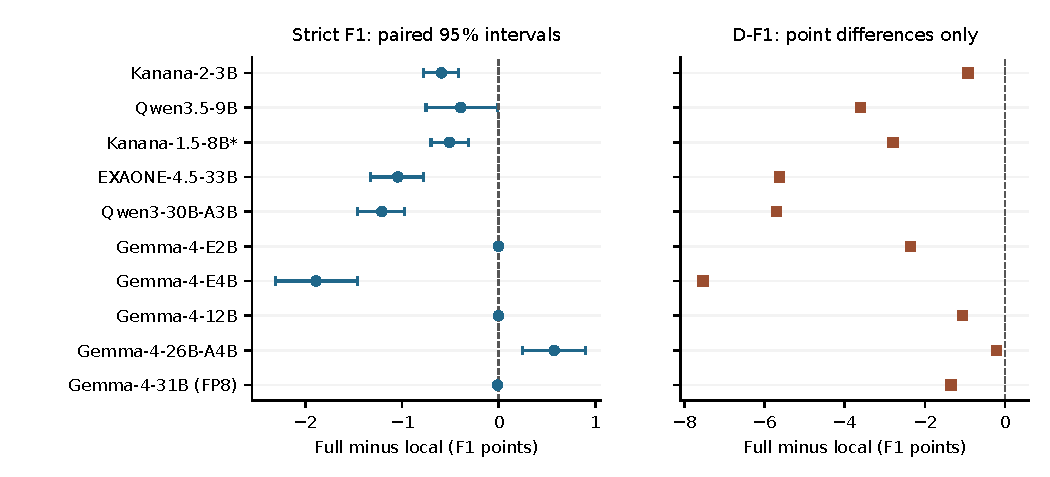
\includegraphics[width=\textwidth]{figures/context-contrasts.pdf}
\caption{Within-model full-minus-local contrasts on each model's original
cohort. Negative values favor local context. Left: strict F1 and pointwise
95\% document-paired bootstrap intervals (2,000 draws, seed 0). Right:
D-F1 point differences; no diagnostic confidence intervals are implied.
*Kanana-1.5-8B uses 1,438 documents; other pairs use 1,440. These are
post-hoc within-model comparisons, not an all-model common-capacity ranking.}
\Description{Two aligned panels show strict F1 differences with intervals
and diagnostic F1 point differences for ten models. Nine strict differences
and all ten diagnostic differences favor local context. Gemma-26B-A4B is
the strict exception. The intervals for Gemma-E2B and Gemma-12B cross zero.}
\label{fig:context-contrasts}
\end{figure*}
